% !TeX root=main.tex

% Different Number of Ports
\begin{figure*}

	\begin{minipage}[b]{.49\textwidth}
		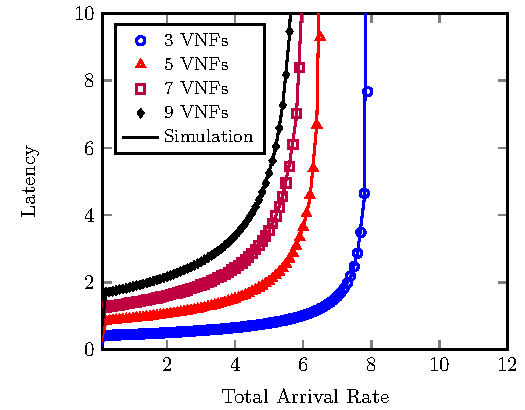
\includegraphics[width=\linewidth]{graphs/diff_lengths}
		\caption{Latency predicted by the model and simulation for a single service with different lengths, $K_i$.}
		\label{fig:length_chain}
	\end{minipage}
	\hfill
	\begin{minipage}[b]{.49\textwidth}
		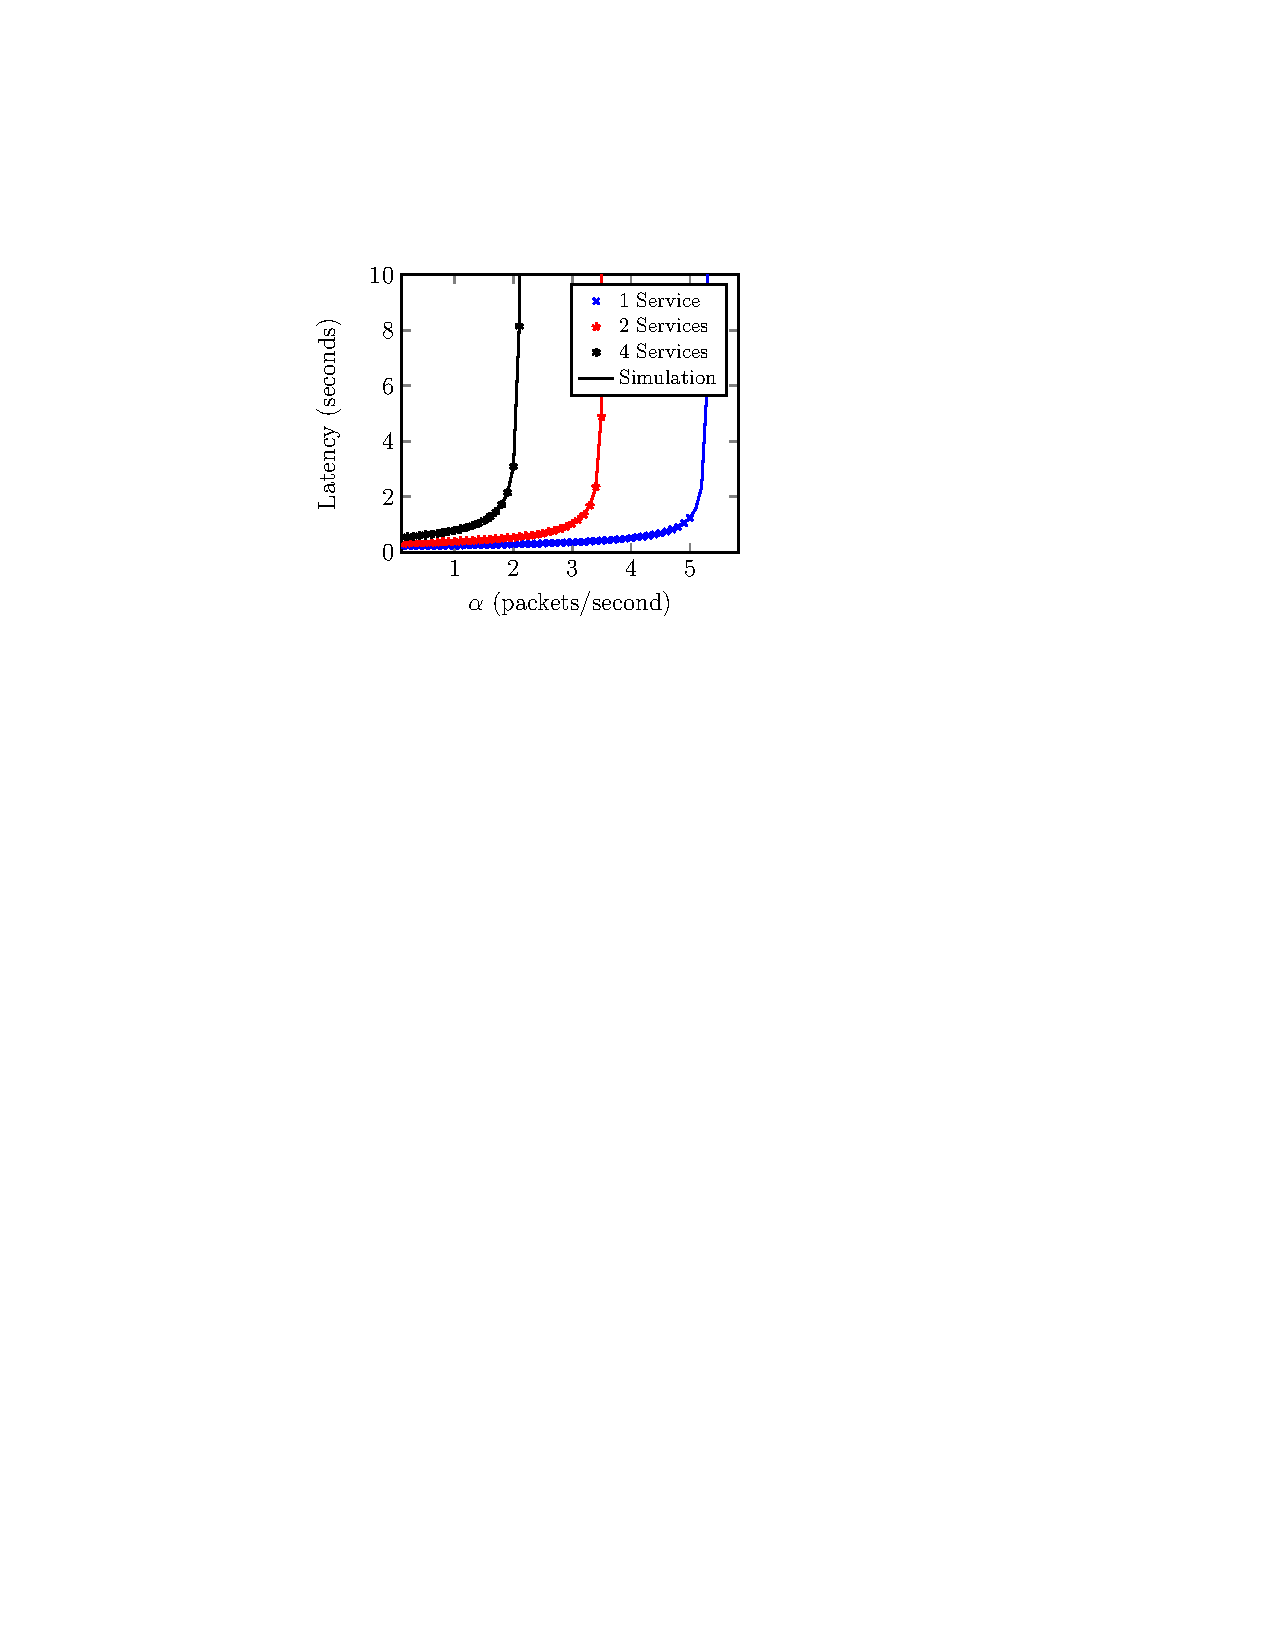
\includegraphics[width=\linewidth]{graphs/mult_services}
		\caption{Latency predicted by the model and simulation for several services ($N_s$)
			with different length service chains, $K_i = 2:(N_s+1)$.}
		\label{fig:mult_services}
	\end{minipage}

	\vspace{2mm}

	\centering
	\begin{minipage}[b]{.49\textwidth}
		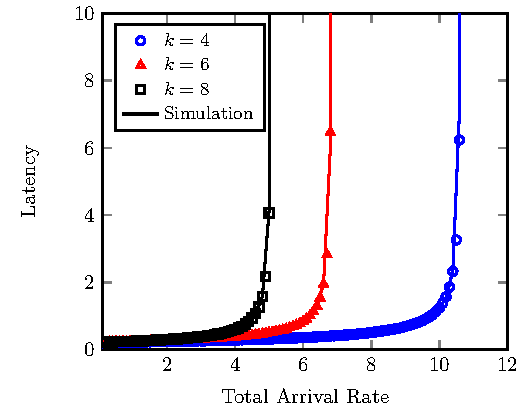
\includegraphics[width=\linewidth]{graphs/num_ports}
		\caption{Latency predicted by the model and simulation for different numbers
			of ports, $k$.}
		\label{fig:num_ports}
	\end{minipage}
	\hfill
	\begin{minipage}[b]{.49\textwidth}
		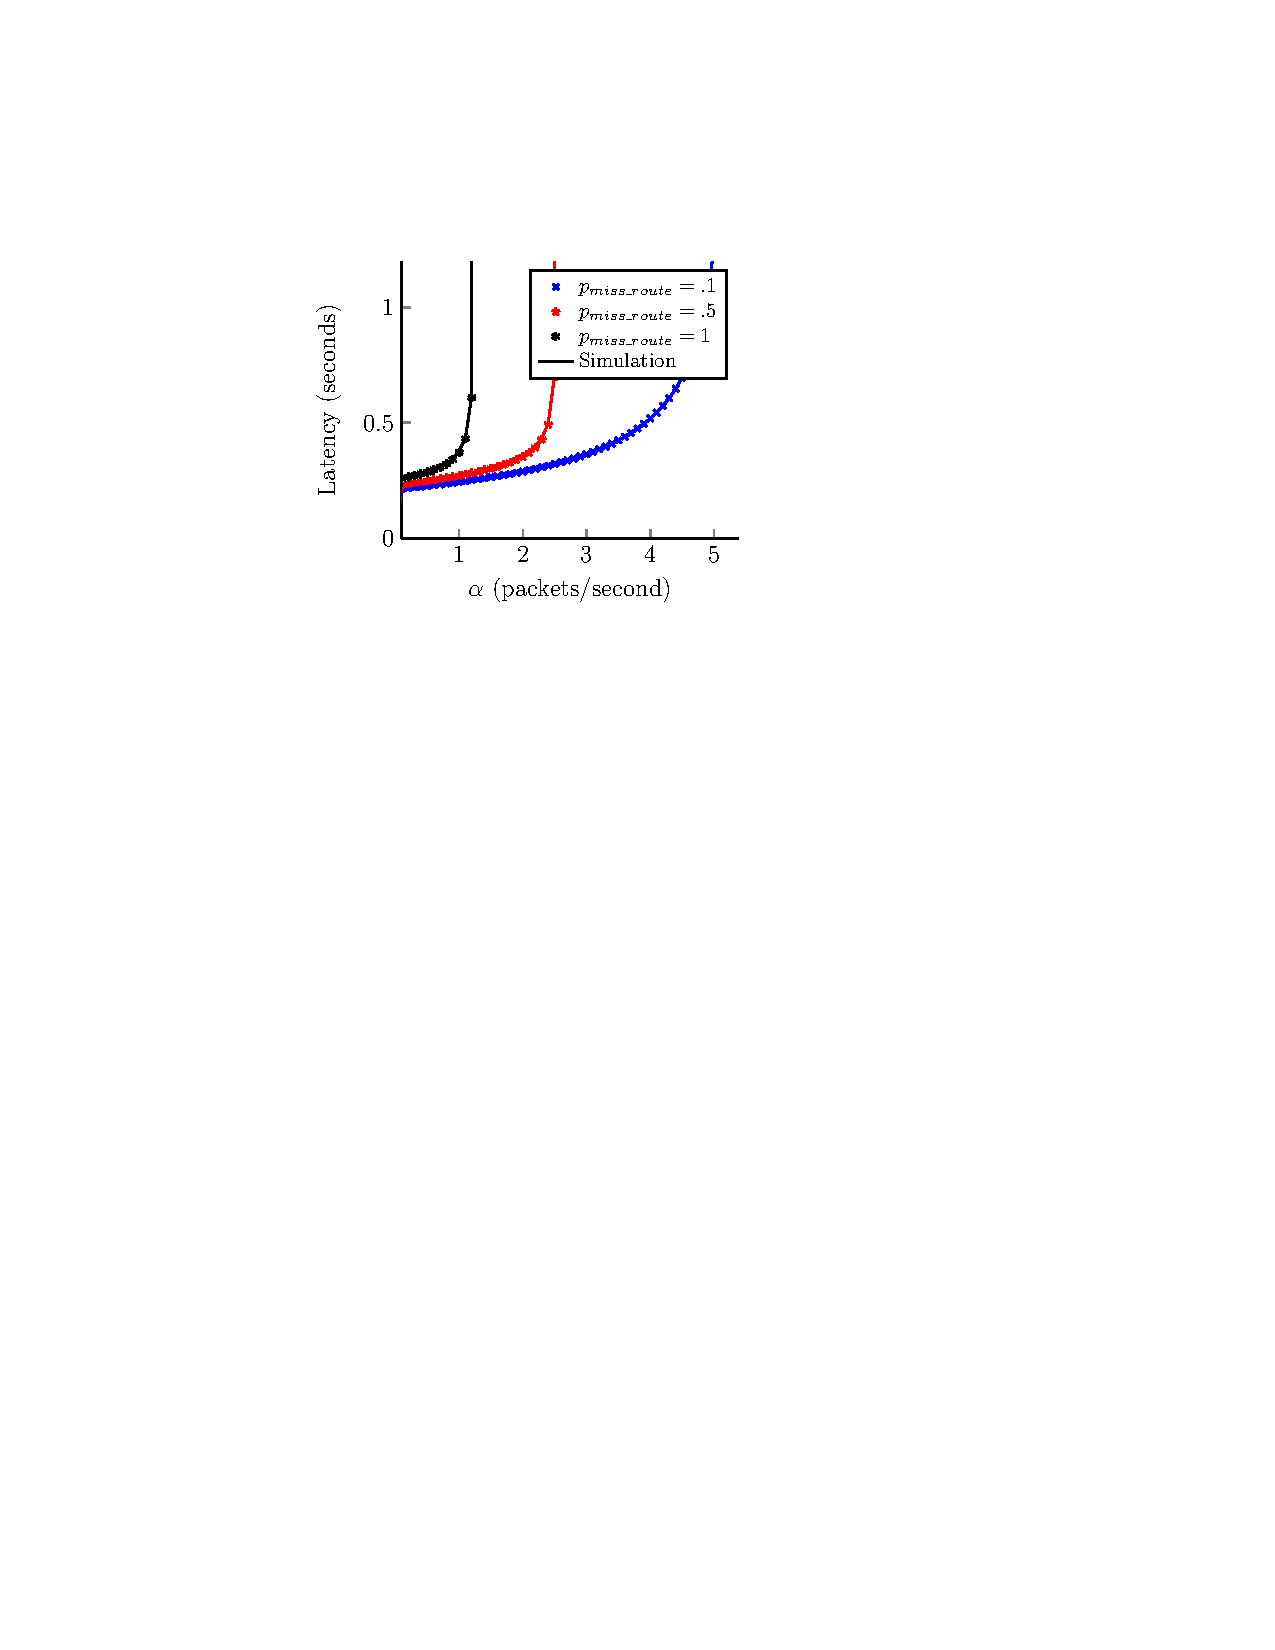
\includegraphics[width=\linewidth]{graphs/diff_sdn}
		\caption{Latency predicted by the model and simulation for different miss rates, $p_{m}$.}
		\label{fig:sdn_perc}
	\end{minipage}

\end{figure*}

\section{Validation and Performance Analysis}
\label{sec:validation}

\subsection{Validation}

To verify the accuracy of the analytical model, a discrete event simulator has been built using OMNeT++ \cite{VargaH08} to simulate a NFV and SDN enabled datacentre network. Each simulation experiment was run until the network reaches its steady state where further network cycles do not change the collected statistics appreciably. Comprehensive simulation experiments were conducted to validate the performance of the proposed analytical model under different network configurations. However for the sake of specific illustration only a selection of tests are presented here and the results comparison between the analytical model and simulation experiments are presented in terms of the average end-to-end latency.

In practice a datacentre can contain on the order of tens of thousands of servers \cite{AWS16}, with each switch supporting 1 to 100Gbits/s traffic a second. It is not feasible to simulate the scale of datacenter network in lab environment. Therefore, a scaled down version of a typical datacentre is modelled. Except where otherwise stated, the following parameters are used in our tests:

\begin{itemize}
	\item $k = 4$, $k_{v} = 2$ and $p_{m} = 0$
	\item The service rate of the switches and SDN controller are set to be 40 packets per second ($\mu_{v} = 40$, $\mu_{c} = 40$)
	\item The service rate of the VNFs is set to be 20 packets per second ($\mu_{f} = 20$)
	\item Services are selected with equal probability
	\item The network holds one service with two VNFs
\end{itemize}

Figs \ref{fig:num_ports} to \ref{fig:mult_services} depict mean message latency predicted by the model plotted against those provided by simulation experiments for a range of parameter settings. For the model, results are only shown where the network is in a steady state, i.e. where the arrival rate is lower than or equal to the service rate for all queues. The figures demonstrate that the simulation results closely match those predicted by the model. The tractability and accuracy of the analytical model make it suitable for analysis of next generation NFV and SDN enabled Mobile Cloud computing datacentres.

\subsection{Performance Analysis}
Finally we can examine the model to establish some conclusions about the datacentre performance under different parameter settings. First we consider the related situations of a different length service and of multiple services of varying lengths. As would be expected, for higher length services as $\lambda$ increases, the waiting time increases greatly such that for services with length of 5 or above the system is only stable for proportionally low arrival rates. From \ref{eq:effective_arrival} we can see that this is a result of packets persisting longer in the network, causing the effective arrival rate to multiply with each increment in the average service length. Correspondingly, we can see that for the case of a multiple services with on average lower service lengths the system is stable for higher relative arrival rate, the key take away is that the limiting factor for capacity in the datacentre is not the number of services but their effective arrival rate.

Next we consider the case of different sized networks. A key assumption in this work is that all VNFs are producing traffic according to the effective arrival rate of the different services. We can see how for larger networks with a correspondingly larger number of VNFs the accumulated arrival rate at different layers causes the expected latency to increase even for small arrival rates. Hence, counterintuitively, larger datacentres that are filled to capacity are not able to provide a better quality of service than a smaller datacenter under the same conditions. From Eqs. \ref{eq:p_vm} to \ref{eq:p_agg_core} we can see this is a consequence of the high probability of packets going via higher levels of the datacentre for larger numbers of ports, hence overloading the higher levels as many packets must traverse all of the network levels. In a practical deployment, datacentre designers must ensure that sequences of VNFs are placed so as to minimise the utilisation of the network.

Finally we consider the case of varying proportions of traffic being sent to the SDN controller. From Fig. \ref{fig:sdn_perc} we can see how a single SDN controller can be overwhelmed even at proportionally low settings of $\lambda$. Considering Eq. \ref{eq:arr_sdn} we see that the arrival rate at the SDN controller receives a proportion of all of the network traffic that is produced by the VNFs. To ensure the SDN controller does not become a bottleneck datacentre designers must ensure that the routing tables in the SDN controllers contain the majority of the information required so that few SDN requests are needed, or that it is significantly more powerful than other servers or must design their topologies to use distribute traffic over multiple SDN controllers.